\documentclass{standalone}
\usepackage{tikz}
\begin{document}
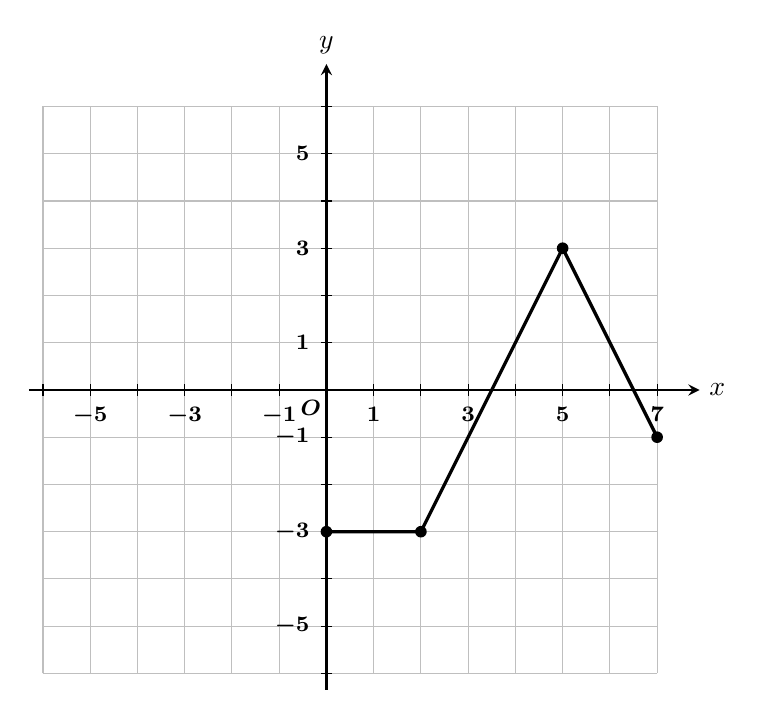
\begin{tikzpicture}[color=black, >=stealth, scale=0.6]
  % Grid: x from -6 to 7, y from -6 to 6
  \draw[gray!50, thin] (-6,-6) grid (7,6);
  % Axes
  \draw[->, thick] (-6.3,0) -- (7.9,0);
  \draw[->, thick] (0,-6.35) -- (0,6.9);
  \node[anchor=west] at (7.9,0) {$x$};
  \node[anchor=south] at (0,6.9) {$y$};
  % Tick marks at every integer
  \foreach \x in {-6,...,-1,1,2,...,7}
    \draw (\x,0.12) -- (\x,-0.12);
  \foreach \y in {-6,...,-1,1,2,...,6}
    \draw (0.12,\y) -- (-0.12,\y);
  % Tick labels (odd values only, as in the original)
  \foreach \x in {-5,-3,-1,1,3,5,7}
    \node[font=\footnotesize\boldmath, anchor=north] at (\x,-0.15) {$\x$};
  \foreach \y in {-5,-3,-1,1,3,5}
    \node[font=\footnotesize\boldmath, anchor=east] at (-0.15,\y) {$\y$};
  \node[font=\footnotesize\boldmath] at (-0.33,-0.38) {$O$};
  % Piecewise-linear graph
  \draw[line width=1.2pt] (0,-3) -- (2,-3) -- (5,3) -- (7,-1);
  % Filled endpoints and vertices
  \foreach \p in {(0,-3), (2,-3), (5,3), (7,-1)}
    \fill[black] \p circle (3.5pt);
\end{tikzpicture}
\end{document}
